\documentclass[11pt]{article}
\usepackage{enumitem}
\usepackage{amsmath,amsthm,amssymb}
\usepackage{color}
\usepackage{tikz}

% Tikz settings optimized for causal graphs.
% Just copy-paste this part
\usetikzlibrary{shapes,decorations,arrows,calc,arrows.meta,fit,positioning}
\tikzset{
    -Latex,auto,node distance =1 cm and 1 cm,semithick,
    state/.style ={ellipse, draw, minimum width = 0.7 cm},
    point/.style = {circle, draw, inner sep=0.04cm,fill,node contents={}},
    bidirected/.style={Latex-Latex,dashed},
    el/.style = {inner sep=2pt, align=left, sloped}
}

\begin{document}
\title{Homework 8}
\author{Brennen Green}
\maketitle


\begin{enumerate}
    \item \begin{enumerate}
        \item Not Reflexive, Not Symmetric, Transitive, Not Anti-Symmetric
        \item Reflexive, Symmetric, Transitive, Not Anti-Symmetric
        \item Not Reflexive, Symmetric, Not Transitive, Not Anti-Symmetric
        \item Not Reflexive, Not Symmetric, Not Transitive, Anti-Symmetric
        \item Reflexive, Symmetric, Transitive, Anti-Symmetric
        \item Not Reflexive, Not Symmetric, Not Transitive, Not Anti-Symmetric
    \end{enumerate}
    \item \begin{enumerate}
        \item \{(1,1), (1,2), (2,1), (2,2), (2,3), (3,1), (3,2), (3,3), (3,4)\}
        \item \{(1,2), (2,3), (3,4)\}
        \item $\emptyset$
        \item \{(1,1), (2,1), (2,2), (3,1), (3,2), (3,3)\}
    \end{enumerate}
    \item \begin{proof}
        \begin{align*}
            & \text{ I. }\\
            & \text{R is reflexive: } (a, a) \in R \\
            & \therefore (a, a) \notin \overline{R} \\
            & \therefore \overline{R} \text{ is irreflexive by definition} \\
            & \text{ II. } \\
            & \text{$\overline{R}$ is irreflexive: } (a, a) \notin \overline{R} \\
            & \therefore (a,a) \in R \\
            & \therefore \text{R is reflexive by definition} \qedhere
        \end{align*}
    \end{proof}
    \item \{(6,1,1,1), (1,6,1,1), (1,1,6,1), (1,1,1,6), (3, 2, 1, 1), (2, 3, 1, 1)
    (3, 1, 1, 2), (3, 1, 2, 1), (1, 3, 2, 1), (1, 3, 1, 2), (1, 2, 3, 1),
    (2, 1, 3, 1), (1, 1, 3, 2), (2, 1, 1, 3), (1, 2, 1, 3), (1, 1, 2, 3)\}
    \item \begin{enumerate}
        \item \{(1,1), (3,1), (2,2), (1,3), (3,3)\}
        \item \{(1,2), (2,2), (3,2)\}
        \item \{(1,1), (1,2), (1,3), (2,1), (2,3), (3,1), (3,2), (3,3)\}
    \end{enumerate}
    \item \begin{enumerate}
        \item 500,500
        \item 1998
        \item 999
        \item 500,500
        \item 1,000,000
    \end{enumerate}
    \item 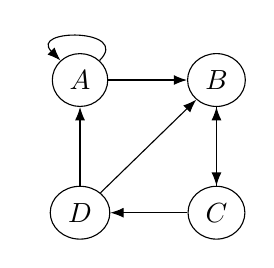
\begin{tikzpicture}
        \node[state] (a) at (0, 0) {$A$};
        \node[state] (b) [right =of a] {$B$};
        \node[state] (c) [below =of b] {$C$};
        \node[state] (d) [below =of a] {$D$};

        \draw (a) to [looseness=3] (a);
        \path (a) edge (b);
        \path (c) edge (d);
        \path (d) edge (b);
        \path (d) edge (a);
        \path (b) edge (c);
        \path (c) edge (b);
    \end{tikzpicture}
    \item If all nodes don't have an edge with themselves
    \item 
        \begin{align*}
            & R \cup \Delta = R \cup \{ (a,a) | a \in A \} \\
            & \{ (a, b) | a \neq b \} \cup \{(a, b) | a = b\}\\
            & \{ (a,b) | a,b \in \mathbb{Z} \} \\
            & = \mathbb{Z} \times  \mathbb{Z}
        \end{align*}
    \item \begin{enumerate}
        \item \{(1,1), (1,2), (1,3), (1,4), (2,1), (2,2), (2,3), (2,4), (3,1),
        (3,2), (3,3), (3,4), (4,1), (4,2), (4,3), (4,4)\}
        \item \{(2,1), (2,3), (2,4), (3,1), (3,3), (3,4), (4,1), (4,3), (4,4)\}
        \item \{(1,2), (1,3), (1,4), (2,3), (2,4), (3,4)\}
        \item \{(1,1), (1,2), (1,3), (1,4), (2,1), (2,2), (2,3), (2,4), (3,1),
        (3,2), (3,3), (3,4), (4,1), (4,2), (4,3), (4,4)\}
    \end{enumerate}
    \item \begin{enumerate}
        \item Equivalence Relation
        \item Isn't Transitive
        \item Isn't reflexive, symmetric, or transitive
        \item Equivalence Relation
        \item Isn't reflexive or transitive
    \end{enumerate}
    \item \begin{enumerate}
        \item $\{y | y \equiv 2(mod 5) \} = \{\dots, -8, -3, 2, 7, 12, \dots\}$
        \item $ \{\dots, -7, -2, 3, 8, 13, \dots\} = \{y|y\equiv 3(mod 5)\}$
        \item $ \{\dots, -9, -4, 1, 6, 11, \dots\} = \{y|y\equiv 6(mod 5)\}$
        \item $ \{\dots, -8, -3, 2, 7, 12, \dots\} = \{y|y\equiv -3(mod 5)\} = \{y|y\equiv 2(mod 5)\}$
    \end{enumerate}
    \item \begin{enumerate}
        \item Poset
        \item Not a Poset
        \item Poset
        \item Not a Poset
    \end{enumerate}
    \item 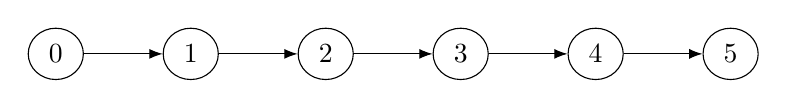
\begin{tikzpicture}
        \node[state] (a) at (0, 0) {$0$};
        \node[state] (b) [right =of a] {$1$};
        \node[state] (c) [right =of b] {$2$};
        \node[state] (d) [right =of c] {$3$};
        \node[state] (e) [right =of d] {$4$};
        \node[state] (f) [right =of e] {$5$};


        \path (a) edge (b);
        \path (c) edge (d);
        \path (b) edge (c);
        \path (d) edge (e);
        \path (e) edge (f);
    \end{tikzpicture}
    \item \begin{enumerate}
        \item Simple Graph
        \item Multigraph
        \item Pseudograph
    \end{enumerate}
    \item No, the sum all the degrees of all vertices is 15 * 5 = 75. This number
    must be twice  the number of edge so 75 = 2n which no integer satisfies
    \item $\frac{\sum_{n = 1}^{v}(n-1)}{2} - c  $
    \item 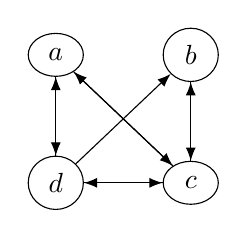
\begin{tikzpicture}
        \node[state] (a) at (0, 0) {$a$};
        \node[state] (b) [right =of a] {$b$};
        \node[state] (c) [below =of b] {$c$};
        \node[state] (d) [below =of a] {$d$};

        \path (a) edge (c);
        \path (a) edge (d);
        \path (b) edge (c);
        \path (c) edge (a);
        \path (c) edge (b);
        \path (c) edge (d);
        \path (d) edge (a);
        \path (d) edge (b);
        \path (d) edge (c);
    \end{tikzpicture}
    \item The two sets are not isomorphic because although they have the same
    number of vertices and edges, the point $u_5$ in the first set does not have
    a point with similar connectivity in the second set
    \item \begin{proof}
        \begin{align*}
            & \text{G is the connected graph of the union } G_1 \cup G_2 \\
            & \text{By definition of a connected graph there must be an edge that} \\
            & \text{connects $v_1 \in G_1$ to $v_2 \in G_1$} \\
            & \therefore \text{There must be a common vertex between $G_1$ and $G_2$} \qedhere
        \end{align*}
    \end{proof}
\end{enumerate}

\end{document}

